\documentclass[10pt]{article}
\usepackage{url,hyperref}
%\usepackage{times}
\usepackage[left=1in,right=1in,top=1in,bottom=1in]{geometry}
\usepackage[utf8]{inputenc}
\usepackage{amsmath, xparse}
\usepackage{graphicx}
\graphicspath{ {./images/} }

\begin{document}

\noindent \textbf{CAP 6640 -- Natural Language Processing\hspace*{\fill}Spring 2025}\\
\noindent{\bf Homework \#4} \hfill Due date: March 6, 2025

%\vspace*{-0.1in}\paragraph{Instructions:}
%Individual work. Cite all references. All submitted assignments must be typed. Using Latex is required. For \LaTeX, you may use your installation, or online IDEs (no installation required); e.g.,  \href{https://www.overleaf.com/}{www.overleaf.com}. Late submissions by at most 24 hours will be scaled down to 50\%; late beyond 24 hours will be worth 0\%. Total of 40 points (+2 bonus). 
\begin{description}
\item[Problem 1:] \hfill %Describe how bidirectional RNNs work, including a diagram and mathematical formulation, and explain the problems they address.

Bidirectional RNN is a special extension standard of RNN architecture that processes input sequences in both forward and backward directions.
This means that each word in the sequence has context from both past and future words.

The key idea is that standard RNNs process text sequentially, meaning each word depends only on the previous words.
This biases the model towards the end of the sentence and makes it difficult to model bidirectional context appearing at the beginning of the sentence.
Bidirectional RNNs address this issue by processing the input sequence in both directions, providing more context for each word.
This mechanism fixes the limited context problem of standard RNNs by incorporating future context, which is necessary for crucial NLP tasks like NER, 
sentiment analysis, speech recognition, and many more.

We can illustrate the working process of bidirectional RNNs with the following diagram:

\begin{figure}[h]
    \centering
    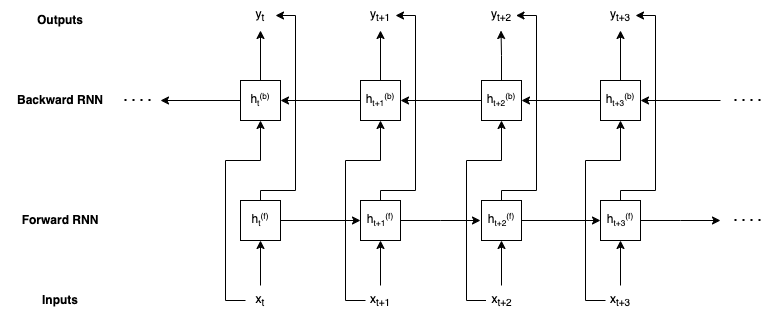
\includegraphics[width=1\textwidth]{biRNN.png}
    \caption{Example of a Bidirectional RNN architecture.}
\end{figure}

A bidirectional RNN consists of two RNNs: Forward RNN, and Backward RNN. 

The forward RNN processes the input sequence from past information to future information, while the backward RNN processes it from 
future information to backward information.
At each time step $t$, both RNNs produce a hidden state $h_t^{(f)}$ and $h_t^{(b)}$, 
where $h_t^{(f)}$ encodes the past context, and $h_t^{(b)}$ encodes the future context.

The final output at each time step is the concatenation of both hidden states as:

\begin{center}
    $h_t = [h_t^{(f)} \oplus h_t^{(b)}]$
\end{center}

where $\oplus$ denotes concatenation operation.

Mathematically, given an input sequence $X = (x_1, x_2, ..., x_T)$, the forward RNN updates its hidden state as:

\begin{center}
    $h_t^{(f)} = f(W_{h}^{(f)}h_{t-1}^{(f)} + W_{x}x_t + b_h^{(f)})$
\end{center}

where $h_t^{(f)}$ is the hidden state of the forward RNN at time step $t$, $W_{h}^{(f)}$ is the weight matrix for the hidden state, $W_{x}$ is the weight matrix for the input, $b_h^{(f)}$ is the bias term, and $f$ is the activation function.

Similarly, the backward RNN updates its hidden state as:

\begin{center}
    $h_t^{(b)} = f(W_{h}^{(b)}h_{t+1}^{(b)} + W_{x}x_t + b_h^{(b)})$
\end{center}

where $h_t^{(b)}$ is the hidden state of the backward RNN at time step $t$, $W_{h}^{(b)}$ is the weight matrix for the hidden state, $W_{x}$ is the weight matrix for the input, $b_h^{(b)}$ is the bias term, and $f$ is the activation function.

The final output of the bidirectional RNN is the concatenation of both hidden states at each time step, which captures both past and future context.

\begin{center}
    $h_t = [h_t^{(f)} \oplus h_t^{(b)}]$
\end{center}

where $\oplus$ denotes concatenation operation, and $h_t$ is the final context-aware representation for each word.

We can list the problems that bidirectional RNNs address as follows:

\begin{enumerate}
    \item Standard RNNs only use past information to predict the next word, which can lead to a short-term bias.
    Bidirectional RNNs incorporate future context, making predictions more accurate.
    \item Long-range dependencies are lost in standard RNNs due to the vanishing gradient problem.
    Bidirectional RNNs capture long-range dependencies by processing the input sequence in both directions.
\end{enumerate}

However, it is important to note that bidirectional RNNs are computationally expensive and require more parameters than standard RNNs, which can make 
training slower and more complex.
Furthermore, bidirectional RNNs are not suitable for real-time applications due to the need to process the entire sequence before making predictions.
Lastly, it still an RNN architecture, which means it is still prone to vanishing gradient problem and struggles with long-range dependencies.

Even though there are some limitations of bidirectional RNNs, they are widely used in NLP tasks like sentiment analysis, NER, and machine translation 
due to their ability to capture bidirectional context effectively as an improvement.

\pagebreak

\item[Problem 2:] \hfill %In the context of CNNs, explain the following concepts with examples: convolution, padding, channels, max pooling, average over time, striding, and k-max pooling. 
 
    \begin{enumerate}
        \item \textbf{Convolution} is the mathematical process of applying a kernel to an input to extract semantic or syntactic features from the given text.
        It involves element-wise multiplication followed by summation. In the context of NLP, convolutions are applied to word embeddings to detect n-gram patterns.
        For example, consider the sentence: "The concert was awesome.". First of all, we embed words into vectors:

        \begin{center}
            "The" $\rightarrow$ [0.1, 0.2, 0.3] \\
            "concert" $\rightarrow$ [0.2, 0.3, 0.4] \\
            "was" $\rightarrow$ [0.3, 0.4, 0.5] \\
            "awesome" $\rightarrow$ [0.4, 0.5, 0.6]
        \end{center}

        Let's assume that we have a kernel of size 2, which is applied to the sentence. The kernel is represented as:

        \begin{center}
            $\displaystyle{\begin{bmatrix} 0.1 & 0.2 & 0.3 \\  0.3 & 0.4 & 0.5 \\ \end{bmatrix}}$
        \end{center}

        The convolution operation is performed as follows:

        \begin{center}
            [0.1, 0.2, 0.3] $\cdot$ [0.1, 0.2, 0.3] + [0.2, 0.3, 0.4] $\cdot$ [0.3, 0.4, 0.5] = 0.1 $\times$ 0.1 + 0.2 $\times$ 0.2 + 0.3 $\times$ 0.3 + 0.2 $\times$ 0.3 + 0.3 $\times$ 0.4 + 0.4 $\times$ 0.5 = 0.01 + 0.04 + 0.09 + 0.06 + 0.12 + 0.2 = 0.52
        \end{center}

        \item \textbf{Padding} involves adding extra zeros or other relevant values around the input to control the output size and preserve sequence length in text.
        For example, without padding the sentence "The concert was awesome.", applying a kernel size of 3 reduces output length from 4 words to 2 words.
        With zero padding, we maintain the original length of the sentence as follows:

        \begin{center}
            "$\phi$" $\rightarrow$ [0.0, 0.0, 0.0] \\
            "The" $\rightarrow$ [0.1, 0.2, 0.3] \\
            "concert" $\rightarrow$ [0.2, 0.3, 0.4] \\
            "was" $\rightarrow$ [0.3, 0.4, 0.5] \\
            "awesome" $\rightarrow$ [0.4, 0.5, 0.6] \\
            "$\phi$" $\rightarrow$ [0.0, 0.0, 0.0] \\
        \end{center}

        \item \textbf{Channels} are the number of feature maps generated by applying multiple kernels to the input. 
        Each channel represents a different feature extracted from the text. This allows to combine different linguistic features.
        For example, if we apply 2 kernels to the sentence "The concert was awesome.", we get 2 channels, each representing a different feature.
        Assume that the other kernel is as follows:

        \begin{center}
            $\displaystyle{\begin{bmatrix} 0.2 & 0.1 & 0.3 \\  0.4 & 0.3 & 0.5 \\ \end{bmatrix}}$
        \end{center}

        For the bigram "The concert", after applying the two kernels, we get two channels for representation as follows:

        \begin{center}
            "The", "concert" $\rightarrow$ [0.52, 0.50] \\
        \end{center}

        \item \textbf{Max Pooling} is a downsampling operation that selects the maximum value from a set of values in a given window while preserving key information.
        This operation helps to capture the most important features. For example, assume that we have the following feature map:

        \begin{center}
            "$\phi$", "The", "concert" $\rightarrow$ [0.52, 0.50] \\
            "The", "concert", "was" $\rightarrow$ [0.48, 0.56] \\
            "concert", "was", "awesome" $\rightarrow$ [0.64, 0.42] \\
            "was", "awesome", "$\phi$" $\rightarrow$ [0.40, 0.38]
        \end{center}

        After applying max pooling for each channel seperately, we get the following representation:

        \begin{center}
            max p $\rightarrow$ [0.64, 0.56] \\
        \end{center}

        \item \textbf{Average Over Time} is a pooling operation that calculates the average of all feature activations across the sequence to capture the overall context.
        This operation helps to reduce the dimensionality of the feature map. Furthermore, averaging them might provide a sentence-level embedding.
        For example, assume that we have the following feature map:

        \begin{center}
            "$\phi$", "The", "concert" $\rightarrow$ [0.52, 0.50] \\
            "The", "concert", "was" $\rightarrow$ [0.48, 0.56] \\
            "concert", "was", "awesome" $\rightarrow$ [0.64, 0.42] \\
            "was", "awesome", "$\phi$" $\rightarrow$ [0.40, 0.38]
        \end{center}

        After applying average over time for each channel seperately, we get the following representation:

        \begin{center}
            avg $\rightarrow$ [0.51, 0.465] \\
        \end{center}

        \item \textbf{Striding} is the process of moving the kernel by a certain number of steps across the input duing convolution to reduce the output size.
        This helps to control computational efficiency and feature map size. When we select stride as 1, the kernel moves one step at a time which outputs a dense feature map.
        For example, assume that we get the following feature map when we apply kernel size of 2 and stride of 1 to the sentence "The concert was awesome.":

        \begin{center}
            "$\phi$", "The", "concert" $\rightarrow$ [0.52, 0.50] \\
            "The", "concert", "was" $\rightarrow$ [0.48, 0.56] \\
            "concert", "was", "awesome" $\rightarrow$ [0.64, 0.42] \\
            "was", "awesome", "$\phi$" $\rightarrow$ [0.40, 0.38]
        \end{center}

        For stride of 2 with the same kernel size, the feature map would be as follows:

        \begin{center}
            "$\phi$", "The", "concert" $\rightarrow$ [0.52, 0.50] \\
            "concert", "was", "awesome" $\rightarrow$ [0.64, 0.42]
        \end{center}

        \item \textbf{K-Max Pooling} selects the top k largest activations values from the feature map instead of a fixed window. 
        This retains significant features while preserving the order of the sequence. For example, assume that we have the following feature map:

        \begin{center}
            "$\phi$", "The", "concert" $\rightarrow$ [0.52, 0.50] \\
            "The", "concert", "was" $\rightarrow$ [0.48, 0.56] \\
            "concert", "was", "awesome" $\rightarrow$ [0.64, 0.42] \\
            "was", "awesome", "$\phi$" $\rightarrow$ [0.40, 0.38]
        \end{center}

        After applying k-max pooling for each channel seperately with k=2, we get the following representation:

        \begin{center}
            k-max p $\displaystyle{\rightarrow \begin{bmatrix} 0.52 & 0.50 \\  0.64 & 0.56 \\ \end{bmatrix}}$
        \end{center}

    \end{enumerate}

\pagebreak

\item[Problem 3:] \hfill %Discuss the operation of multi-layer RNNs, highlighting the advantages of using multiple layers and identifying four key challenges associated with them.

A multi-layer RNN consist of multiple stacked RNN layers where the output of one layer is fed as input to the next layer.
This hierarchical architecture allows the network to learn complex patterns and dependencies in the data across different levels of abstraction.

For an in input sequence $X = (x_1, x_2, ..., x_T)$, a single-layer RNN updates its hidden state as:

\begin{center}
    $h_t^{(1)} = f(W_{h}h_{t-1}^{(1)} + b_h)$
\end{center}

where $h_t^{(1)}$ is the hidden state of the first layer at time step $t$, $W_{h}$ is the weight matrix, $b_h$ is the bias term, and $f$ is the activation function.

What multi-layer RNNs do is to extend this formulation to multiple layers. In a multi-layer RNN, each hidden state at layer $l$ takes input from the previous layer's hidden state as

\begin{center}
    $h_t^{(l)} = f(W_{h}^{(l)}h_t^{(l-1)} + b_h^{(l)})$
\end{center}

where $h_t^{(l)}$ is the hidden state of the $l$-th layer at time step $t$, $W_{h}^{(l)}$ is the weight matrix, $b_h^{(l)}$ is the bias term, and $f$ is the activation function.

This enhances representation learning, allowing the network to learn hierarchical representations of the input data, where each layer processes information at a different level of abstraction, with lower layers 
capturing local patterns and deeper layers modeling high-level dependencies.

The advantages of using multiple layers in RNNs include:

\begin{enumerate}
    \item \textbf{Hierarchical Representation Learning:} As mentioned earlier, multi-layer RNNs can learn hierarchical representations of the input data.
    Lower layers capture local patterns like words in a phrase, while deeper layers capture long-term dependencies like sentence meaning.
    \item \textbf{Increased Model Capacity:} Compared to single layer RNNs, multi-layer RNNs can model complex sequential data better than shallow alternatives.
    \item \textbf{Improved Generalization:} Hierarchical feature extraction of multi-layer RNNs makes the useful for complex sequences like a long text and speech.
\end{enumerate}

However, multi-layer RNNs also face several challenges:

\begin{enumerate}
    \item \textbf{Vanishing and Exploding Gradients:} Like in every RNN architecture, as gradients propagate through many layers and time steps, 
    they become exponentially small, preventing earlier layers from learning.
    \item \textbf{Long-Term Dependency:} Even though multi-layer RNNs are better than shallow ones, they still struggle to capture long-term dependencies in the data due to 
    the vanishing gradient problem, which can limit their ability to model sequences with long-range dependencies.
    \item \textbf{Computational Complexity and Cost:} Having multiple RNNs means more model parameters to train, which can require significant computational resources, 
    making training slow.
    \item \textbf{Optimization Challenges:} Training multi-layer RNNs can be challenging due to overfitting and convergence of gradients, which can make it harder to 
    find an optimal model configuration.
\end{enumerate}

\pagebreak

\item[Problem 4:] \hfill %Explain the encoder-decoder architecture, detailing its working mechanism and providing three real-world applications.

The encoder-decoder architecture is a Seq2Seq model used for mapping an input sequence to an output sequence of varying lengths.
The key idea is that the encoder processes the input sequence and generates a fixed-length context vector, which is then fed to the decoder to generate the output sequence.
It is commonly used in speech recognition, text summarization, and machine translation tasks.
The model consists of two parts: the encoder and the decoder.

The encoder takes the input sequence $X = (x_1, x_2, ..., x_T)$ and generates a hidden representation at each step.
The final hidden state $h_T$ is passed to the decoder as a fixed-length context vector $C$.
As an encoder architecture, RNNs, LSTM or GRU can be used.
Mathematically, the encoder processes the input seqeunce $X$ word by word as follows:

\begin{center}
    $h_t = f(W_{h}h_{t-1} + W_{e}x_t + b_h)$
\end{center}

where $h_t$ is the hidden state at time step $t$, $W_{h}$ is the weight matrix for the hidden state, $W_{e}$ is the weight matrix for the input, $b_h$ is the bias term, and $f$ is the activation function.

After $x_T$ is processed, the final hidden state $h_t$ is passed to the decoder as a compressed representation of $X$.

The decoder takes the context vector $C$ and generates the output sequence $Y = (y_1, y_2, ..., y_T)$.
It predicts each word step by step, using the previous output word as input for the next prediction.
This will continue until an end-of-sequence token is generated.
Like in the encoder, RNNs, LSTM or GRU can be used as the decoder architecture.
Mathematically, the decoder updates its hidden state as:

\begin{center}
    $s_t = f(W_{d}y_{t-1} + U_{d}s_{t-1} + V_{d}C + b_h)$
\end{center}

where $s_t$ is the hidden state at time step $t$, $W_{d}$ is the weight matrix for the output, $U_{d}$ is the weight matrix for the hidden state, $V_{d}$ is the weight matrix for the context vector, $b_h$ is the bias term, and $f$ is the activation function.

The output sequence $Y$ is generated by applying a softmax function to the hidden state $s_t$ at each time step.
This ensures that the model remembers context while generating each word.

However, the compression of the input sequence into a fixed-length context vector can lead to information loss for long sentences.

Three real-world applications of the encoder-decoder architecture are:

\begin{itemize}
    \item \textbf{Machine Translation:} The encoder-decoder architecture is widely used in machine translation tasks to convert text from one language to another.
    The encoder processes the input sentence in the source language and generates a context vector, which is then passed to the decoder to generate the translated sentence in the target language.
    With this way, we learn contextual dependencies better than phrase-based translation.
    \item \textbf{Speech Recognition:} The encoder-decoder architecture is used in speech recognition tasks to convert spoken language into text.
    The encoder processes the audio input and generates a context vector, which is then passed to the decoder to generate the corresponding text output. 
    \item \textbf{Text Summarization:} The encoder-decoder architecture is used in text summarization tasks to generate a short summary of a longer text.
    The encoder processes the input text and generates a context vector, which is then passed to the decoder to generate the summary. This captures key information while removing redundancy.
\end{itemize}

\pagebreak

\item[Problem 5:] \hfill %Explain how CNNs are applied to text understanding tasks, such as sentiment analysis.

CNNs are widely used in text understanding tasks, such as sentiment analysis, due to their efficient way of capturing local patterns in a sentence without 
requiring sequential processing. 

Assume that we have a sentence "I absolutely love this movie! It was fantastic." and we want to classify the sentiment of this sentence.
The words "love", "fantastic", and "absolutely" suggest strong positive sentiment, and the CNN model should be able to scan key phrases like "was fantastic" to
determine the sentiment of the sentence. CNNs can work very well in this scenario since the main job is to detect local patterns or n-grams in text and classify the 
sentiment efficiently.

The first step in applying CNNs to text understanding tasks is to convert words into numerical representations.
Assume that we have the following word embeddings for the sentence "I love this amazing movie!":

\begin{center}
    "I" $\rightarrow$ [0.2, 0.1, 0.5, 0.7] \\
    "love" $\rightarrow$ [0.8, 0.3, 0.6, 0.5] \\
    "this" $\rightarrow$ [0.4, 0.9, 0.2, 0.8] \\
    "amazing" $\rightarrow$ [0.7, 0.5, 0.3, 0.6] \\
    "movie" $\rightarrow$ [0.9, 0.6, 0.4, 0.7] \\
\end{center}

The next step is to apply convolutional operations to the word embeddings to detect
local patterns or n-grams in the sentence. For example, assume that we have a kernel of size 2 that is applied to the sentence.
The kernel to detect bigrams is represented as:

\begin{center}
    $\displaystyle{\begin{bmatrix} 0.1 & 0.2 & 0.3 & 0.4 \\  0.5 & 0.4 & 0.3 & 0.2 \\ \end{bmatrix}}$
\end{center}

We will slide over word pairs in the sentence and apply the convolution operation to detect bigrams.
For instance, the convolution operation for the bigram "love this" is as follows:

\begin{center}
    [0.8, 0.3, 0.6, 0.5] $\cdot$ [0.1, 0.2, 0.3, 0.4] + [0.4, 0.9, 0.2, 0.8] $\cdot$ [0.5, 0.4, 0.3, 0.2] = 0.8 $\times$ 0.1 + 0.3 $\times$ 0.2 + 0.6 $\times$ 0.3 + 0.5 $\times$ 0.4 + 0.4 $\times$ 0.5 + 0.9 $\times$ 0.4 + 0.2 $\times$ 0.3 + 0.8 $\times$ 0.2 = 1.44
\end{center}

After applying the convolution operation to all possible bigrams in the sentence, we get a feature map as 

\begin{center}
    [1.25, 1.44, 1.39, 1.57]
\end{center}

Each value represents how strongly a phrase contributes to sentiment.
We can see that this filter activates strongly for "amazing movie" bigram, which suggests a positive sentiment in the sentence.

After convolution, we have a feature map showing how strongly different phrases contribute to sentiment.
The next step is to apply max pooling to the feature map to keep the most important phrases.
For example, after applying max pooling with a window size of 2, we get the following representation:

\begin{center}
    max p $\rightarrow$ [1.44, 1.57]
\end{center}

This ensures the model focuses on key phrases like "love this" and "amazing movie".

Finally, we can pass the output of max pooling to a fully connected layer and a softmax function to classify the sentiment of the sentence.

\begin{center}
    $y = softmax(W \times [1.44, 1.57] + b)$
\end{center}

With this example, we can see how CNNs can be applied to text understanding tasks like sentiment analysis by capturing local patterns in the text efficiently.
The same mechanism of CNNs can be applied to other text understanding tasks like text classification and more.

\pagebreak

\item[Problem 6:] \hfill %Describe how neural machine translation operates and compare it to alternative approaches.

Neural machine translation, NMT in short, is a deep learning-based approach that translates text from one language to another using NNs.
Unlike traditional rule-based or statistical machine translation methods, NMT learns language patterns automatically from large datasets.

The key components of NMT are the encoder and the decoder, which are connected by an attention mechanism for improved performance.
The encoder processes the input sentence and generates a context vector, which is then passed to the decoder to generate the output sentence.
Attention mechanism helps the model to focus on relevant parts of the input sentence while generating the output. It is especially useful for long sentences.
Instead of using a single context vector, attention computes weights for each input word dynamically.

The encoder takes the input sentence $X = (x_1, x_2, ..., x_T)$ and generates a hidden representation at each step.

\begin{center}
    $h_t = f(W_{h}h_{t-1} + W_{e}x_t + b_h)$
\end{center}

The final hidden state $h_T$ is passed to the decoder as a fixed-length context vector $C$.

For example, we want to tranlate the sentence "I love dogs!" from English to Turkish.
The encoder processes the input sentence and generates a context vector $C$ as

\begin{center}
    $[2.1, -1.3, 0.9, 1.4]$
\end{center}

The decoder takes the context vector and generates the target sentence word by word.
At each step, it predicts the next word based on the previous words and the context vector as:

\begin{center}
    $s_t = f(W_{d}y_{t-1} + U_{d}s_{t-1} + V_{d}C + b_h)$
\end{center}

For instance, the decoder generates the first word "Ben" in Turkish conditioned on the $C$.
Then, it generates the next word "köpekleri" based on the previous word "Ben" and updated $s_t$.
This process continues until the end-of-sequence token is generated. 
Finally, the decoder generates the output sentence "Ben köpekleri seviyorum!".

Compared to other machine translation approaches like statistical machine translation (SMT) and rule-based machine translation (RBMT), NMT has several advantages:

\begin{itemize}
    \item RBMT relies on hand-crafted rules and dictionaries, which can be time-consuming and error-prone to create.
    SMT uses statistical models to translate text, which can be computationally expensive and require large amounts of data.
    NMT, on the other hand, learns translation patterns automatically from data using deep learning techniques.
    \item RBMT Requires linguistic expertise to create rules and dictionaries, which can be challenging for low-resource languages.
    SMT relies on large bilingual datasets that may not capture complex language patterns well.
    NMT needs a very large monolingual and bilingual datasets to learn translation patterns effectively.
    \item RBMT produces rigid translations based on predefined rules, which may not capture nuances in the language.
    SMT can produce better fluent translations but they are mostly limited to phrase-based translations.
    NMT can generate more fluent and natural translations by learning contextual dependencies and capturing long-range dependencies.
\end{itemize}

\pagebreak

\item[Problem 7:] \hfill %Identify three limitations of RNNs that CNNs overcome.

\begin{enumerate}
    \item \textbf{Prefix Dependency Issue:} RNNs process text sequentially, meaning each word depends only on the previous words.
    This biases the model towards the end of the sentence and makes it difficult to model bidirectional context appearing at the beginning of the sentence.
    For instance, for the sentence "The academic article I read yesterday was illuminating.", RNNs may struggle to capture the relationship between "academic article" and "illuminating"
    as it is difficult to accurately predict long-range dependencies. 
    CNNs do not rely on sequential dependencies. 
    Instead, they apply convolution filters over all n-grams at once, allowing the model to capture context from any part of the input.
    This makes CNNs better at capturing global context, rather than being biased toward words at the end of the sentence.
    \item \textbf{Overweighting of Recent Tokens:} Because of gradient updates, RNNs tend to give more weight to recent words while forgetting earlier ones, 
    which leads to a short-term bias. This makes RNNs over-reliant on recent tokens when predicting the next word.
    For example, in the sentence "I love dogs, but I am allergic to them.", RNNs may struggle may give too much weight to "allergic", ignoring "love" and leading to a wrong negative
    prediction.
    CNNs, on the other hand, apply equal-weight convolutional filters across the text, meaning they treat all words equally rather than favoring recent ones.
    Furthermore, max-pooling helps select the most relevant features from anywhere in the sequence, avoiding overemphasis on recent words.
    \item \textbf{Softmax at the Last Step:} In RNNs, the softmax function is applied only at the final step, meaning earlier states do not directly 
    contribute to the prediction. This loses intermediate information and makes it difficult to capture long-term dependencies.
    To give an example, assume we have partially generated the sentence "The Orlando weather today is ..." and we want to predict the next word.
    Since softmax is only applied at the last step, important features from earlier time steps such as "Orlando" and "weather" may be weakened, 
    leading to an incorrect next word prediction.
    On contrary, CNNs apply multiple filters at every step, ensuring that intermediate representations contribute equally to the final prediction.
    Instead of relying on a single softmax output, CNNs aggregate features at multiple layers, improving word prediction accuracy.
\end{enumerate}

\end{description}

\end{document}